\section{Translations}

\begin{frame}{\secname}
  $\sim$3000 source strings translated into 14 languages by 59 contributors
  \textcolor{red}{\faHeart}

  \begin{center}
    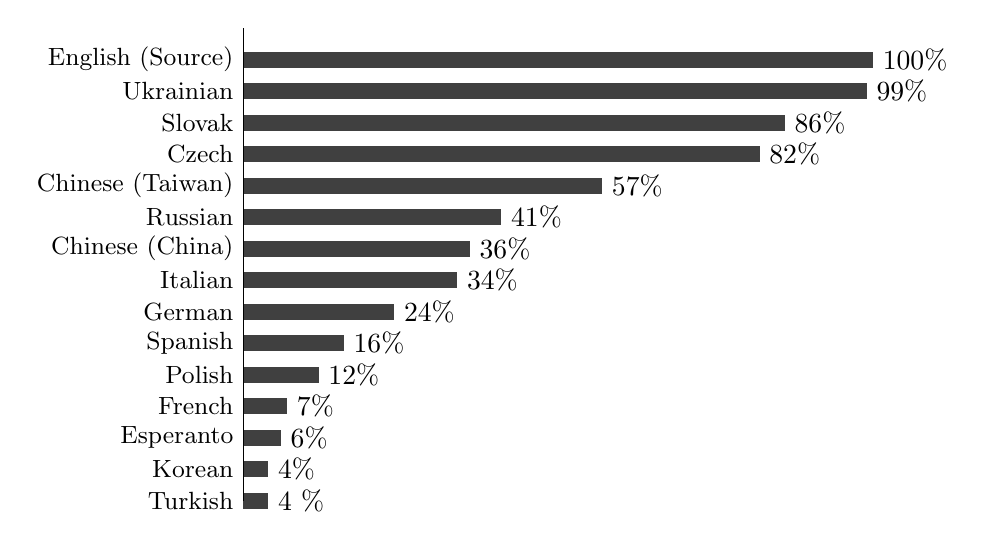
\begin{tikzpicture}[x=0.08cm,y=-0.4cm]
      \foreach \l/\x[count=\y] in {
        English (Source)/100,
        Ukrainian/99,
        Slovak/86,
        Czech/82,
        Chinese (Taiwan)/57,
        Russian/41,
        Chinese (China)/36,
        Italian/34,
        German/24,
        Spanish/16,
        Polish/12,
        French/7,
        Esperanto/6,
        Korean/4,
        Turkish/4
      }
      {
        \node[left] at (0,\y) {\small{\l}};
        \fill[darkgray] (0,\y-.25) rectangle (\x,\y+.25);
        \node[right] at (\x, \y) {\x\%};
      }
      %\draw (0,0) -- (100,0);
      %\foreach \x in {20, 40, ..., 100}
      %{
      %  \draw (\x,.2) -- (\x,0) node[below] {\x};
      %}
      \draw (0,0) -- (0,15);

      %\onslide<2>{
      %  \node at (70,10) {\Huge{Thanks! \Smiley}};
      %}

    \end{tikzpicture}
  \end{center}
\end{frame}

\note{
  Translations into languages other than English are continuously growing
  as well. At the moment, LibrePCB is available at least partially in 13
  different languages, contributed by 42 translators.\\

  A big thank-you to the translators for your work!
}
